\documentclass[10pt]{beamer}
\usepackage[utf8]{inputenc}
\usepackage[dvipsnames]{xcolor}
\usepackage{charter}
\usepackage{amsmath}
\usepackage{amsfonts}
\usepackage{mathtools}
\usepackage{amssymb}
\usepackage{hyperref}
\usepackage[ruled,vlined]{algorithm2e}
\usepackage{commath}

\title{Variance reduced methods in Deep Neural Networks}
\author{Alexander Apostolov}
\institute {Ecole Polytechnique Fédérale de Lausanne}
\date{November 11th 2020}

\begin{document}


\frame{\titlepage}


\begin{frame}{Goal of this semester project}

Analyze the effect of \alert{variance reduction methods} in \alert{deep neural networks}.
\newline
\begin{itemize}
    \item Analysis of SGD, Adam, AdaGrad, SVRG and STORM on a small NN.
    \item Analysis and trying to get insights about possibilities of using better performance of variance reduction methods on deep neural networks. 
\end{itemize}
    
\end{frame}

\begin{frame}
\frametitle{Why variance reduction methods?}
\begin{itemize}
    \item In machine learning, the following optimization is often encountered:\
    Let $f_1, f_2, \dots, f_n$ be a sequence of vector functions from $\mathbb{R}^d$ to $\mathbb{R}$.
    The goal is to find a solution to the following optimization problem:
    $$\min F(w),~~F(w)=\frac{1}{n}\sum_{i=1}^n f_i(w)$$
    \item \textbf{Gradient Descent (GD)} is a standard method to solve this:
    $$w^{(t)} = w^{(t-1)} - \eta_t \nabla F(w^{(t-1)})$$
    \item Each iteration requires computation of the whole gradient, this is why \textbf{Stochastic Gradient Descent (SGD)} which decrease computational cost by $\frac{1}{n}$ per iteration has been widely adopted:
    $$w^{(t)} = w^{(t)} -\eta_t \nabla f_{i_t}(w^{(t-1)})$$
\end{itemize}
\end{frame}

\begin{frame}{Why variance reduction methods?}
    Randomness in SGD introduces variance which slows down convergence. This creates a trade off between fast per iteration computation and fast convergence.
    
    \vspace{5mm}
    \textbf{Variance reduced methods} allows keeping fast convergence at fast per iteration speed. We will analyze two methods:
    \begin{itemize}
        \item \textbf{Stochastic Variance Reduced Gradient (SVRG)}
        \item \textbf{STOchastic Recursive Mometum STORM}
    \end{itemize}
    
\end{frame}

\begin{frame}{SVRG}
    Each iteration of SVRG is given by:
    $$w^{(t)} = w^{(t)} -\eta_t(\nabla f_{i_t}(w^{(t-1)}) - \nabla f_{i_t}(\Tilde{w}) + \Tilde{\mu})$$
    where $\Tilde{w}$ is snapshot of $w$ we make every $m$ iterations and :
    $$\Tilde{\mu} = \nabla F(\Tilde{w}) = \frac{1}{n}\sum_{i=1}^n \nabla f_i(\Tilde{w})$$
    
    Notice that: 
    \begin{itemize}
        \item $\nabla f_{i_t}(w^{(t-1)}) - \nabla f_{i_t}(\Tilde{w}) + \Tilde{\mu}$ is an unbiased estimate of $\nabla P(w)$:
    $$\mathbb{E}[w^{(t)} | w^{(t-1)}] = w^{(t-1)}-\eta_t \nabla F(w^{(t-1)})$$
        \item Variance is reduced. When $\Tilde{w}$ and $w^{(t)}$ both converge to $w_{\ast}$, then $\Tilde{\mu} \rightarrow 0$. If $\nabla f_i(\Tilde{w}) \rightarrow \nabla f_i(w_{\ast})$, then:
        $$\nabla f_i(w^{(t-1)}) - \nabla f_i(\Tilde{w}) + \Tilde{\mu} \rightarrow \nabla f_i(w^{(t-1)}) - \nabla f_i(w_{\ast}) \rightarrow 0$$
    \end{itemize}
\end{frame}


\begin{frame}{SVRG}
    \begin{algorithm}[H]
        \DontPrintSemicolon
        \SetAlgoNoLine

        \KwIn{learning rate $\eta$ and update frequency $m$}
        \textbf{Initialize} $\Tilde{w}_0$\;
        \For{$s \leftarrow 1, 2, \dots$}{
          $\Tilde{w} \gets \tilde{w}_{s-1}$\;
          $\Tilde{\mu} \gets \frac{1}{n}\sum_{i=1}^n \nabla f_i(\Tilde{w})$\;
          $w_0 \gets \tilde{w}$\;
          \For{$t \leftarrow 1,2\dots, n$}{
            Randomly pick $i_t \in \{1, \dots, n\}$  
            
            $w^{(t)} \gets w^{(t)} -\eta(\nabla f_{i_t}(w^{(t-1)}) - \nabla f_{i_t}(\Tilde{w}) + \Tilde{\mu})$
          }
          \textbf{Save snapshot} $\tilde{w}_s \gets w_m$\;
        }
        \caption{{\textsc{SVRG Procedure}}}
        \label{algo:svrg}
    \end{algorithm}
\end{frame}

\begin{frame}{STORM}
    Each iteration of STORM is given by:
    $$d^{(t)} = (1-a)d^{(t-1)} + a\nabla f_{i_t}(w^{(t)}) + (1-a)(\nabla f_{i_t}(w^{(t)}) +  \nabla f_{i_t}(w^{(t-1)}))$$
    $$w^{(t+1)} = w^{(t)} - \eta d_t$$
    Notice that:
    \begin{itemize}
        \item When $w^{(t)} \approx w^{(t-1)}$, then the last term of the first equality tends to 0. Then the update is exactly the same as SGD with momentum. 
    \end{itemize}
\end{frame}

\begin{frame}{STORM}
    \begin{algorithm}[H]
        \DontPrintSemicolon
        \SetAlgoNoLine

        \KwIn{Hyperparameters $k, w, c$}
        \textbf{Initialize} $w_1$\;
        $G_1 \gets \norm {\nabla f_{i_1}(w_1)}$\;
        $d_1 \gets \nabla f_{i_1}(w_1)$\;
        \For{$t \leftarrow 1, 2, \dots$}{
          $\eta_t  \gets \frac{k}{(w+\sum_{i=1}^tG_t^2)^{1/3}}$\;
          $w_{t+1} \gets w_t - \eta_t d_t$\;
          $a_{t+1} \gets c\eta_t^2$\;
          $G_{t+1} \gets \norm{\nabla f_{i_{t+1}}(w_{t+1})}$\;
          $d_{t+1} \gets \nabla f_{i_{t+1}}(w_{t+1}) + (1-a_{t+1})(d_t - \nabla f_{i_{t+1}}(w_t))$\;
        }
        \caption{{\textsc{STORM Procedure}}}
        \label{algo:storm}
    \end{algorithm}
\end{frame}


\begin{frame}{SVRG vs STORM}
\begin{itemize}
    \item Both algorithms need two gradient computations per iteration.
    \item SVRG needs a full gradient computation every m steps (every 5 epochs in non-convex problems).
    \item difficult to get insight on hyperparameters $k,w \text{ and } c$ in STORM.
    \item More hyperparameters to tune for STORM.
\end{itemize}
\end{frame}

\begin{frame}{Cross-validation for Hyperparameter selection}
    We performed 4-Fold cross-validation on MNIST with LeNet:
    \begin{itemize}
        \item \textbf{Adam} : gridsearch for $\eta \in \{10^{-5}, 10^{-4}, 10^{-3}, 0.01, 0.1\}$ \newline
        Best value : $\eta = 10^{-4}$
        \item \textbf{SGD} : gridsearch for $\eta \in \{10^{-5}, 10^{-4}, 10^{-3}, 0.01, 0.1\}$ \newline
        Best value : $\eta = 0.1$
        \item \textbf{AdaGrad} : gridsearch for $\eta \in \{10^{-4}, 10^{-3}, 0.01, 0.1\}$ \newline
        Best value : $\eta = 0.1$
        \item \textbf{SVRG} : gridsearch for $\eta \in \{10^{-5}, 10^{-4}, 10^{-3}, 0.01, 0.1\}$ \newline
        Best value : $\eta = 0.01$
        \item \textbf{STORM} : gridsearch for $c \in \{10^{-5}, 10^{-4}, 10^{-3}, 0.01, 0.1\}$ and $k \in \{10^{-3}, 0.01, 0.1, 1\}$\newline
        Best value : $c = 100$ and $k=0.1$
        
    \end{itemize}
\end{frame}

\begin{frame}{Cross-validation for Adam}
    \begin{figure}
        \centering
    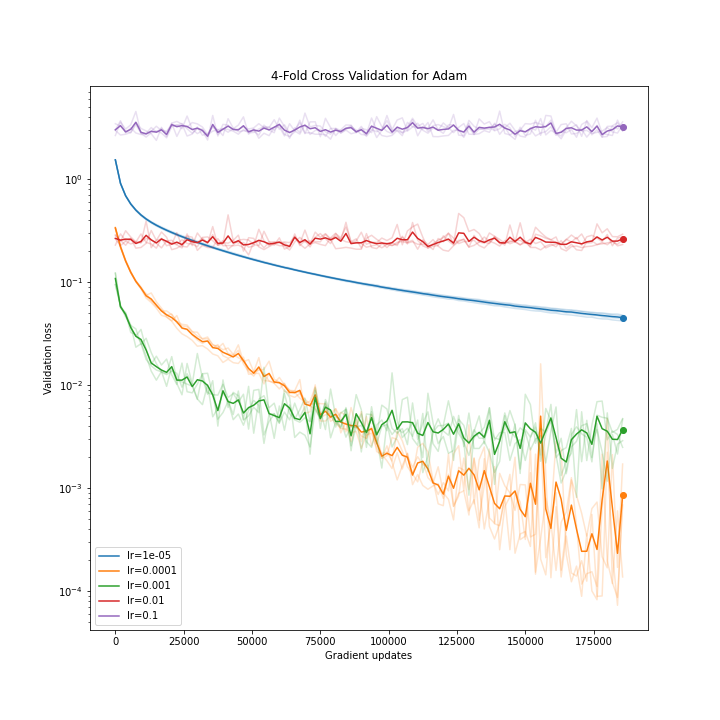
\includegraphics[scale=0.35]{midterm presentation/images/adamCV.png}
        \label{fig:adamCV}
    \end{figure}   
\end{frame}

\begin{frame}{Algorithm comparison on MNIST}
    \begin{figure}
        \centering
    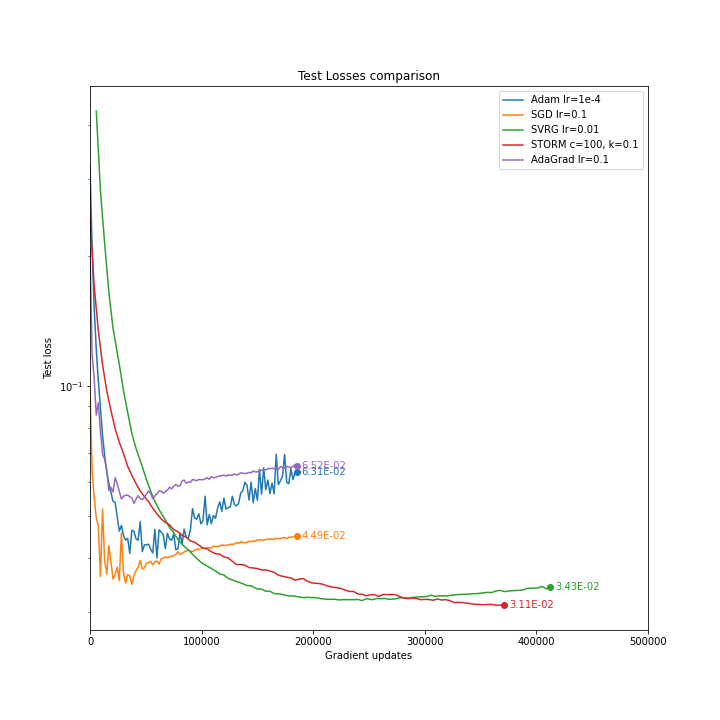
\includegraphics[scale=0.35]{midterm presentation/images/testLossesMnist.png}
        \label{fig:testLossesMnist}
    \end{figure}   
\end{frame}
####explain CV setup

####Show results

###Paper about ineffectiveness

###setup to test this

####replace Batch-norm by Init



\begin{frame}{ }
\begin{center}
     \Huge Any questions?
\end{center}
   
\end{frame}

\end{document}

